% TEMPLATE for Usenix papers, specifically to meet requirements of
%  USENIX '05
% originally a template for producing IEEE-format articles using LaTeX.
%   written by Matthew Ward, CS Department, Worcester Polytechnic Institute.
% adapted by David Beazley for his excellent SWIG paper in Proceedings,
%   Tcl 96
% turned into a smartass generic template by De Clarke, with thanks to
%   both the above pioneers
% use at your own risk.  Complaints to /dev/null.
% make it two column with no page numbering, default is 10 point

% Munged by Fred Douglis <douglis@research.att.com> 10/97 to separate
% the .sty file from the LaTeX source template, so that people can
% more easily include the .sty file into an existing document.  Also
% changed to more closely follow the style guidelines as represented
% by the Word sample file. 

% Note that since 2010, USENIX does not require endnotes. If you want
% foot of page notes, don't include the endnotes package in the 
% usepackage command, below.

% This version uses the latex2e styles, not the very ancient 2.09 stuff.
\documentclass[letterpaper,twocolumn,10pt]{article}
\usepackage{endnotes}
\usepackage{alltt}
\usepackage{url}
\usepackage{amsfonts}
% Type1 fonts please!
\usepackage{amsmath}
\usepackage[T1]{fontenc}
%\usepackage{times,courier,mathptmx}
\usepackage{pifont}
\usepackage{times}
\usepackage{textcomp}
\usepackage{graphicx}
%\usepackage{amsmath,amsthm}
\usepackage{epsfig}
\usepackage{cite}
%\usepackage{color}
\usepackage[table]{xcolor}
\usepackage{xspace}
%\usepackage[tight]{subfigure}
\usepackage{mathspec}
\usepackage[subrefformat=parens,labelformat=parens]{subfig}
\setmainfont[Ligatures=TeX,BoldFont={Minion Pro Bold}, 
 ItalicFont={Minion Pro Italic},
 BoldItalicFont={Minion Pro Bold Italic}]{Minion Pro}
\setmathrm{Minion Pro} 
\setmathfont{Minion Pro}
\setmathfont(Digits,Latin){Minion Pro}
\begin{document}

\newcommand{\notegk}[1]{\textcolor{red}{[G: #1]}}
\newcommand{\noteion}[1]{\textcolor{blue}{[I: #1]}}
%don't want date printed
\date{}

%make title bold and 14 pt font (Latex default is non-bold, 16 pt)
\title{\huge \textit{The Theory of Wait Times}}

%for single author (just remove % characters)
%\author{
%{\rm A1}\\
%UC Berkeley
%\and
%{\rm A2}\\
%UC Berkeley
%\and
%{\rm A3}\\
%UC Berkeley
%} % end author

\maketitle

% Use the following at camera-ready time to suppress page numbers.
% Comment it out when you first submit the paper for review.
%\thispagestyle{empty}


\subsection*{Abstract}
Your Abstract Text Goes Here.  Just a few facts.
Whet our appetites.

\section{Introduction}

Internet services like web video-search follow strict real-time constraints. 
Services running on large-amount of data leverage massive parallelism to meet these deadlines. 
This parallelism is achieved by employing partition-aggregate workflow where a particular request is handled by thousands of machines, 
each one of them operating on a shard of data; the responses being aggregated 
in a hierarchical fashion before the final response is computed.


This partition-aggregate workflow may involve multiple stages, e.g., while the web-search application operates on a two level 
aggregation tree, workloads like video-search or news-search do away with only a single stage. 
%We focus on these two type of applications, one requiring a single stage and others requiring two stages to 
%compute the final result. 
This distinction results in two types of deadlines, hard and soft deadlines. \notegk{explain properly, why hard/soft or remove.}
The real-time constraints manifest themselves as a latency budget that the highest-level aggregator has.
%; either the single aggregator for a single-stage workflowimpose a soft-deadline over the entire workflow and this latency target is subject to optimisation. 
For the 1-stage case, the aggregator may have more freedom to make this dynamically tune 
if it feels that the response may come back by a small amount of additional waiting.
The aggregation nodes in the middle of partition-aggregate pipeline, however, are encumbered by hard deadlines that denote how long should they wait to collect all the sub-responses
before sending the results up in the hierarchy. These deadlines are hard since a higher level aggregator may just ignore the responses of the lower-level aggregators if they arrive late.
% if an upper stage decides to stop waiting, then responses that have not yet been
%received are no longer of use.
\begin{figure}[!t]
\centering
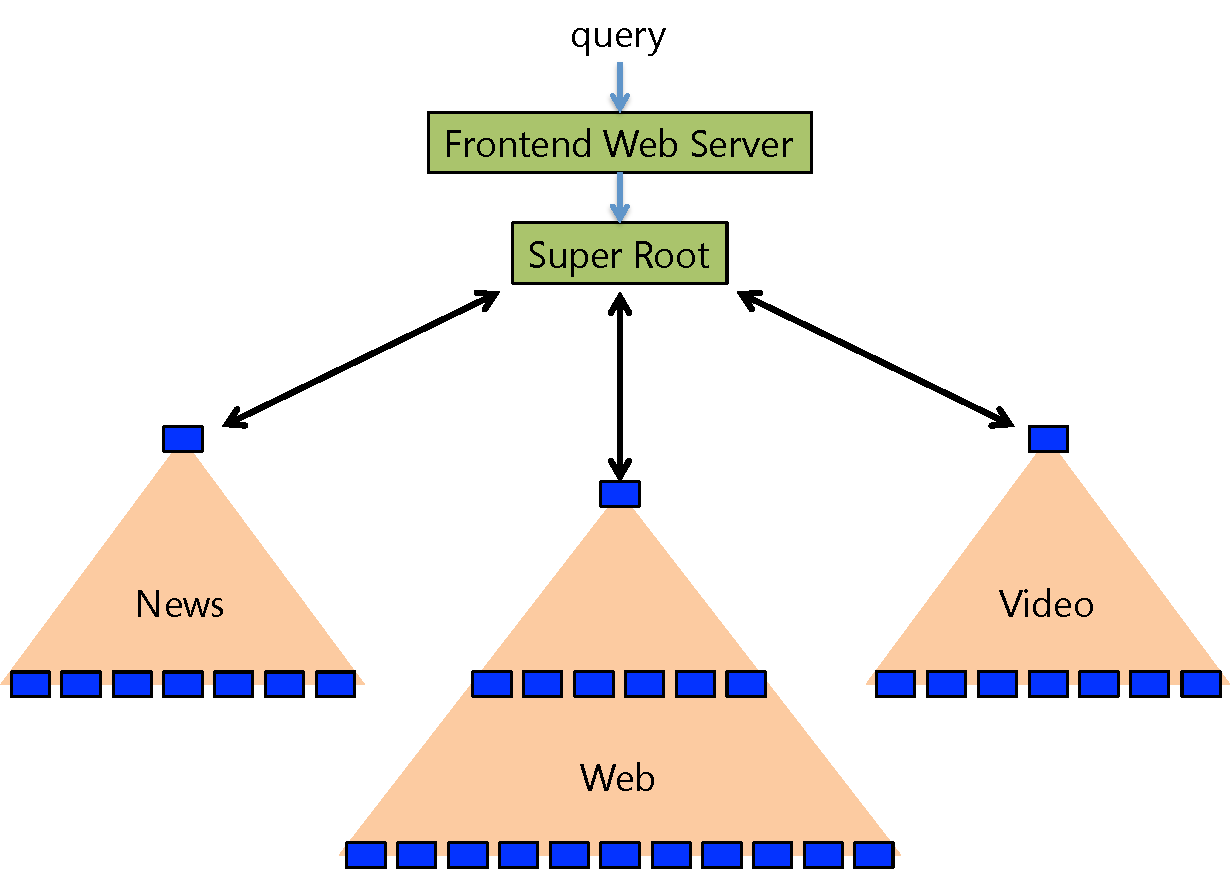
\includegraphics[width=3in]{Figures/Services.pdf}
\label{figure:Services}
\caption{\small A few online services. \notegk{From Jeff Dean's talk.}}
\end{figure}

\begin{figure*}[t]
  \centering
  \subfloat
  {
    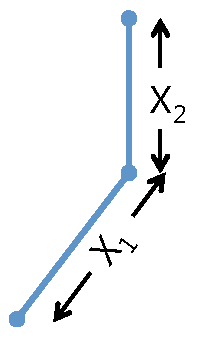
\includegraphics[width=1in]{Figures/2Stage.pdf}
    \label{figure:2StageSimple}
  }
  \hspace{0.5in}
  \subfloat
  {
    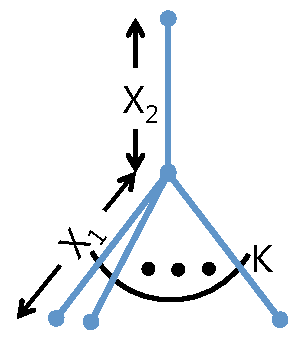
\includegraphics[width=1.5in]{Figures/2StageAggregation.pdf}
    \label{figure:2StageAggregation}
  }
  \hspace{0.5in}
    \subfloat
  {
    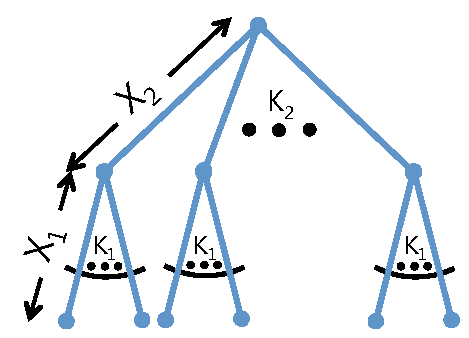
\includegraphics[width=2.5in]{Figures/2StageAggregationFull.pdf}
    \label{figure:2StageAggregationFull}
  }
    \caption{A simple two-stage pipeline. (a) Without aggregation (b) With aggregation at the first stage (c) With aggregation at both the stages.}
  \label{figure:2Stage}
\end{figure*}

Given the heavy-tailed distributions for task durations prevalent in data centers, 
the aggregator may need to ship out partial results in order to either meet the latency budget
(as in the 1-stage case) or to make sure the set of responses get included in the final result 
delivered by the higher-level aggregator (as in the 2-stage case). This creates a tradeoff between waiting for additional time to gather more responses or to send partial results in order to be collected by the higher-level aggregator. In this paper, we focus on the above trade-off and formalise it.

\section{Analysis}
Consider a simple two-stage pipeline as shown in Figure~\ref{figure:2Stage}. 
Figure~\ref{figure:2StageSimple} denote the two stages in the pipeline without any aggregation. 
Let $X_1$ and $X_2$ be random variables denoting the time taken in the first and the second stages of the pipeline respectively. 
%The CDF for $X_1$ is denoted by $\phi_{X_1}(t)$ which is equal to the probability, $\mathbb{P}[X_1 \leq t]$, and the corresponding density function given by $p_1(t)$.
%The distribution for the end-to-end response time is given by the $Y = X_1 + X_2$ whose CDF, denoted by $\phi_{Y}(t)$, is given by:
%$$
%\phi_Y(t) = \int_{y = 0}^t \ \int_{x_1 = 0}^{y} p_1(x_1) \  p_2(y - x_1) \ dx_1 \  dy
%$$
%For the sake of simplicity, let us assume that $X = X_1 = X_2$. If $X$ is exponentially distributed with parameter $\lambda$, then $\phi_Y(t) = (1 - (1 + \lambda t) e^{-\lambda t})$
%with $p_Y(t) = \lambda^2 t e^{-\lambda t}$.

%When the responses from the first stage are aggregated, the time that the first stage takes is distributed as per $X_1' = \textsf{max}(X_1^1, X_1^2, \dots, X_1^k)$. 
%The end-to-end response time variation is then given by, $Z = X_1' + X2$. 
%If $X_1$ is exponentially distributed, as above, then $\phi_{X_1'}(t)$ is given by $(1 - e^{-\lambda t})^k$ with $p_{X_1'} = k\lambda(1 - e^{-\lambda t})^{k- 1}e^{-\lambda t}$.
%The CDF, $\phi_Z(t)$ is given by:
%$$
%\phi_Z(t) = \int_{z = 0}^t \ \int_{x_1' = 0}^{y} p_1(x_1') \  p_2(z - x_1') \ dx_1' \  dz
%$$
%which becomes the integral of an incomplete Beta function.

%The exponential distributions reflect the long tail in task durations that occur in typical data center applications. 
The aggregator needs to wait for all the responses to come back before ranking them and sending them up the chain.
Since this operates under the regime of tight latency targets, if all the responses do not come back in time, the aggregator may decide to leave some of them and rank the partial set of responses thereby degrading the quality\footnote{We use a generic term, information content, to denote the quality of the result. \notegk{To fix.}}. We ask the following question - Given a budget, $D$, for the end-to-end latency, how much should individual stage aggregators wait before sending their partial result up the chain. We formalise the tradeoff between the quality of result and meeting the deadline target in this paper. 
%To the best of our knowledge, we are the first to undertake an analysis of such workflow and the formalism that follows. \\
\subsection{A simple model}
Consider the aggregator stage having waited for $t$ units of time and has not received all the responses.
Denote $N(t)$ to be the random variable denoting the number of responses received uptil time $t$. 
For a particular branch, the probability that the aggregator receives that response is
$\mathbb{P}[X_1 \leq t] = \phi_{X_1}(t)$.
Therefore, $N(t)$ is binomial with success probability $ = \phi_{X_1}(t)$. 
The expected number of responses received by time $t$, thus, is given by $\mathbb{E}[N(t) = k\phi_{X_1}(t)$.
For exponentially distributed $X_1$, this is given by $k(1 - e^{-\lambda t})$. 
These set of responses contribute to the final result if the aggregator meets the deadline $D$ of the above stage which happens with probability $\phi_{X_2}(D - t)$. 
Thus while $\mathbb{E}[N(t)]$ is an increasing function in $t$, the probability that those set of responses make it in time to be aggregated by the top level decreases with time.
If lost, the entire branch of computation is lost. It is important for internet services to deliver all the responses, and the quality of query is of utmost importance. 
Thus one can write the Utility function, $U(t)$, as $\mathbb{E}[N(t)]\phi_{X_2}(D - t) = k\phi_{X_1}(t)\phi_{X_2}(D - t)$. 
If $X_1$ and $X_2$ are exponentially distributed, then $U(t)$ = $k(1 - e^{-\lambda_1 t})(1 - e^{-\lambda_2(D - t)})$.
The function being concave exhibits a distinct maxima when $U'(t) = k\left(\phi_{X_1}'(t)\phi_{X_2}(D - t) - \phi_{X_1}(t)\phi_{X_2}'(D - t)\right) = 0$
It is to be noted that for this simple model, the value of $t$ that maximizes $U(t)$ is independent of the fanout, $k$, for the workflow.
%Two important points surface, one is that this timeout selection is independent of the fanout degree, $k$. 
%Even if the expected utility small, one can make the most out of it.
%The curve becomes flatter as one increases the latency budget.

\begin{figure}[!t]
\centering
\subfloat[Exponential Distribution] {
  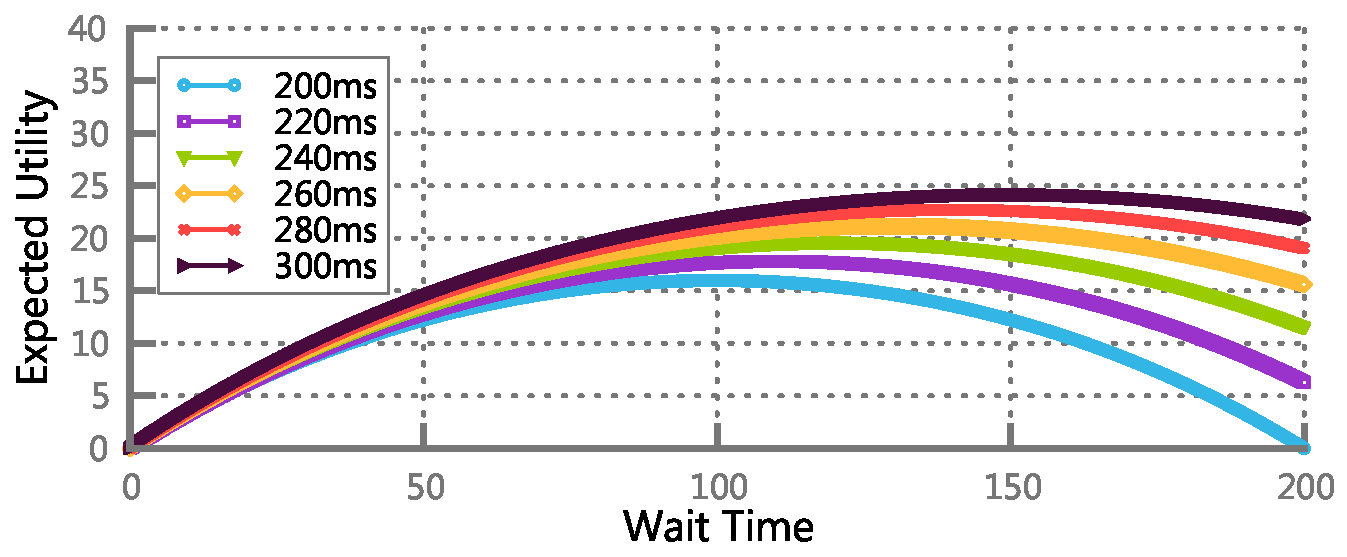
\includegraphics[width=3.1in]{Matplotlib/UtilityAnalyticalExp.pdf}
  \label{figure:UtilityAnalyticalExp}
}
\vspace{0.1in}
\subfloat[Normal Distribution] {
	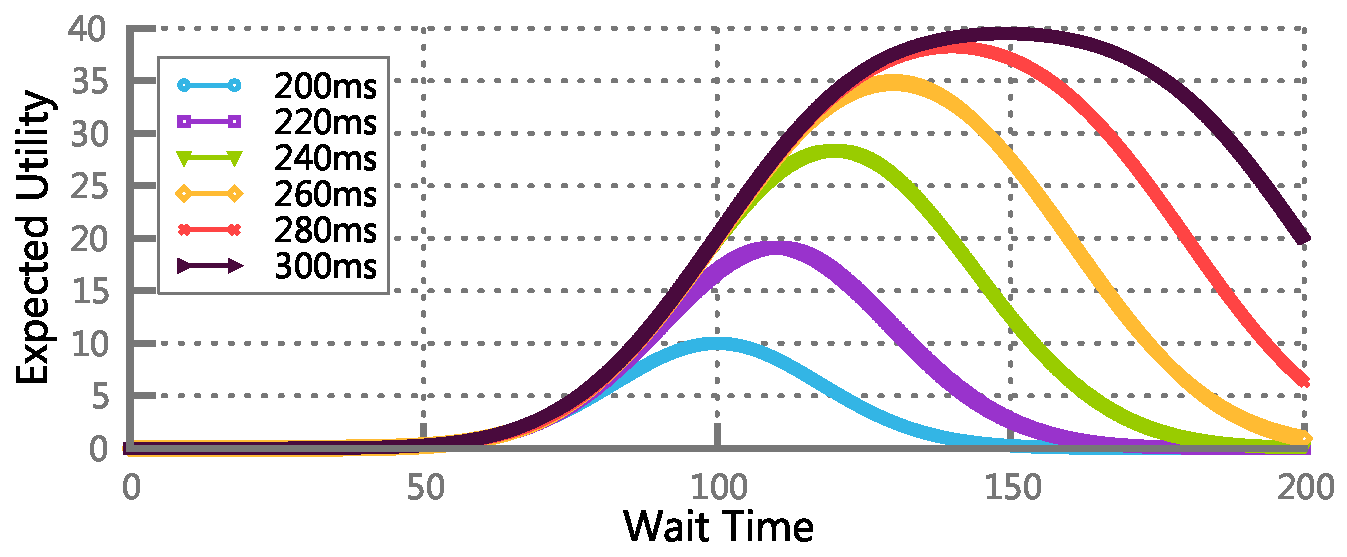
\includegraphics[width=3in]{Matplotlib/UtilityAnalyticalNormal.pdf}
	\label{figure:UtilityAnalyticalNormal}
}
\caption{\small Utility function values as a function of wait time $t$ for different deadline, $D$, values. for a) exponentially distributed, and b) normally distributed, $X_1$ and $X_2$, with mean 100ms.}
\end{figure}

Let $X_1$ and $X_2$ both have a mean of 100ms.%\notegk{Numbers from D3}
Figure~\ref{figure:UtilityAnalyticalExp} and figure~\ref{figure:UtilityAnalyticalNormal} show the the variation of the expected utility with respect to the wait time at the aggregator node for different deadline values both for exponential and normal distribution for task times respectively. The exponential distributions, due to the long tail have flatter utility curves and considerably lower values in expectation. The normal distributions on the other hand

For the entire partition-aggregate tree as shown in Figure~\ref{figure:2StageAggregationFull}, the utility function becomes $k_1 k_2 \phi_{X_1}(t)\phi_{X_2}(D - t)$ and therefore, the maxima is still independent of both $k_1$ and $k_2$. 

\subsection{In-depth analysis}
The above discussion omits the fact that there are only a finite number of responses that an
aggregator has to collect and thus, there is a finite probability that it receives all the
responses before timing out, which is given by $\phi_{X_1}^{k}(t)$, where $t$ is the timeout. Thus, we revisit the problem statement with this perspective.
Consider, again, the aggregator having waited for $t$ units of time and not having received 
all the responses.
Note that now, since the prior is that the aggregator has not received all responses in time $t$, the only decision is whether to wait for an additional $\Delta t$ time or not.
The tradeoff with regards to waiting for some more time is as follows; 
there is a non-zero probability that it receives additional responses in this time, 
but this comes at the expense of increased probability of missing the latency target,
 or worse, getting missed by the aggregator at the above stage, 
making that entire branch of computation wasted.
The probability a particular branch sends back its response in the 
additional $\Delta t$ time = $p = \textsf{Pr}[t \leq X_1 \leq (t + \Delta t)] = (\phi_{X_1}(t + \Delta t) - \phi_{X_1}(t))$. 
Thus, the number of responses received in time $\Delta t$ is 
binomial with success probability $p$ and with expectation $kp$. 
These responses add to the utility function if they reach the high-level aggregator in time, which happens with probability $\phi_{X_2}(D - (t + \Delta t))$. 
Thus, the expected gain due to these additional responses is given by $k(\phi_{X_1}(t + \Delta t) - \phi_{X_1}(t))\phi_{X_2}(D - (t + \Delta t))$.
However, this additional waiting might cause the responses received uptil now to 
not be included in the final result if the second-stage deadline is missed. As discussed, previously the expected number of responses received till time $t$ is $k\phi_{X_1}(t)$. 
The probability that the second stage deadline is missed due to the additional waiting
is $\mathbb{P}[D - t > X_2 > D - (t + \Delta t)] = \phi_{X_2}(D - t) - \phi_{X_2}(D - (t + \Delta t))$. Thus, the expected loss in the value of utility is $k\phi_{X_1}(t)\phi_{X_2}(D - t) - \phi_{X_2}(D - (t + \Delta t))$. However, this loss only occurs when all the responses have not been collected by the aggregator which happens with probability $(1 - \phi_{X_1}^{k}(t))$.
The net overall change is then $k(\phi_{X_1}(t + \Delta t) - \phi_{X_1}(t))\phi_{X_2}(D - (t + \Delta t)) - k\phi_{X_1}(t)()\phi_{X_2}(D - t) - \phi_{X_2}(D - (t + \Delta t))(1 - \phi_{X_1}^{k}(t))$.
%The expected gain to the utility function 
%Given that the aggregator has waited for $t$ units of time, the probability \textsf{Pr}[A new response is received in $\Delta t$ | Elapsed time $= t$] = $1 - $\textsf{Pr}[No new response arrives in $\Delta t$ | Elapsed time $= t$] = $1 - \left[1 - (\phi_{X_1}(t + \Delta t) - \phi_{X_1}(t)) \right] ^k$. 
One can find the derivative of the utility function by computing $\lim_{\Delta t \to 0} \frac{\Delta U(t)}{\Delta t}$. Note that the maxima is no longer independent of $k$, but varies very little with it. \notegk{Include analysis.}


\begin{figure}[t]
\centering
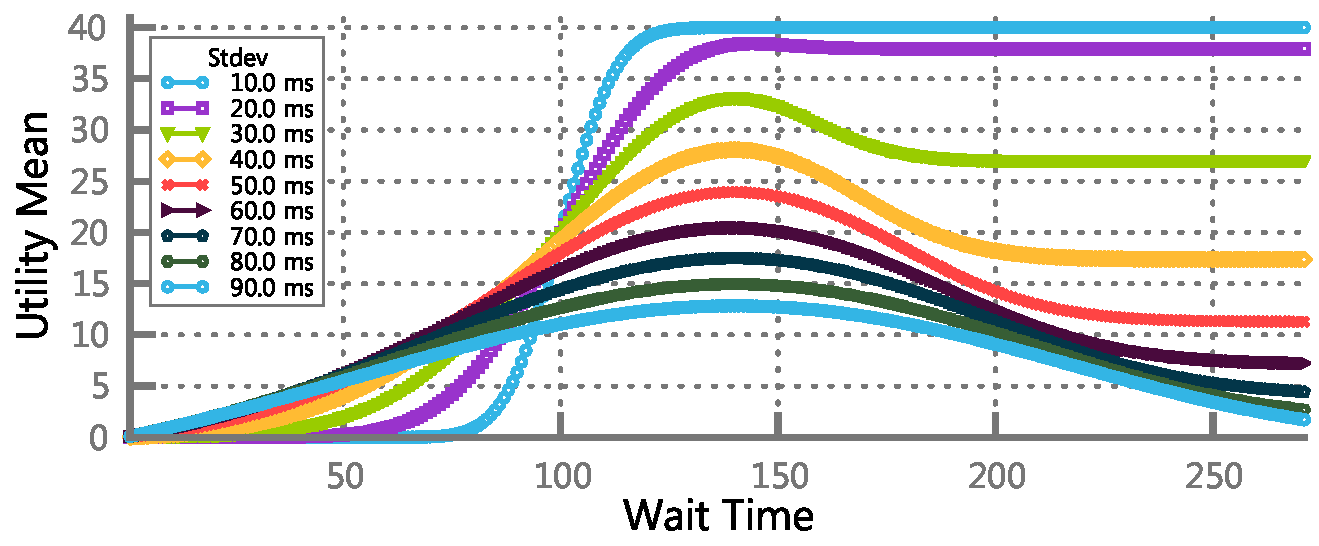
\includegraphics[width=3.2in]{../VrikshaSim/Results/09-01-2013/CheckDeltaUAnalysis.pdf}
\caption{\small Expected utility obtained from the analytical model for normal distribution of task times for various values of standard deviation.}
\label{figure:NormalProperAnalytical}
\end{figure}

We plot this analytical model for a normal distribution by keeping the mean of both the stages as 100ms and varying the standard deviation from 10ms to 90ms. Figure~\ref{figure:NormalProperAnalytical} shows the value of expected utility with this model.
When the variance in the system is low, then having a large value of timeout is not much worse much than the optimal value since there is a good chance that the timeout doesn't get triggered (since all the responses come before it). But when the variance in the system is more, then choosing a suitable timeout becomes critical for performance.


\subsection{Alternate Analysis}
\notegk{The above discussion omits the fact that there are only a finite number of responses that an aggregator has to collect and thus, there is a finite probability that it receives all the responses without timing out. Consider the scenario in Figure~\ref{figure:2StageAggregationFull} and  assume that the aggregator is using a time-out, $t$ to wait for all the responses. Let $V$ denote the random variable corresponding to the maximum of the response times of individual branches, i.e., $V = \textsf{max}(X_1, X_2, \dots, X_K)$. Since all the responses are received, the utility is either K or 0 depending upon whether the second stage is able to meet the deadline. Thus the contribution to the expected response quality of this case is given by:
$$
U_1(t) = \int_{\tau = 0}^t \ p_V(\tau)\ k\ \phi_{X_2}(D - \tau)\ d\tau
$$
The probability that all the responses are not received by time $t$ is $(1 - \phi_{V}(t))$. The expected number of responses in this case is $\mathbb{E}[N(t) | N(t) \neq k]$ and thus the contribution of this case to the expected utility is:
$$
U_2(t) = k\ \left(\phi_{X_1}(t) - \phi_{X_1}^k(t)\right) \phi_{X_2}(D - t)
$$
The overall expected utility is given by $U(t) = U_1(t) + U_2(t)$ and the optimisation to maximise $U(t)$ is not independent of $k$.
}


\section{Algorithm}
\subsection{Same distribution for all tasks}
In this section, we consider the case when each request is equally expensive and thus the task durations are spread similarly across all requests. Thus, one need to tune a single value for the time-out at the mid-level aggregator and the end-to-end deadline to maximize . 
In this section, we outline a simple algorithm to select time-out values for aggregation based workloads under a tight latency budget. The next section discusses an online variant of the algorithm that addresses many assumptions made in this section. In particular, we assume we assume that all the requests follow the same distribution for task durations.

\notegk{Algorithm}

\subsection{Request-specific distribution of task durations}
Different requests take different amount of times. 
For the web-search workload, some queries are more complex than the 
other and thus take more time on average than others. 
One can think of the following two cases.

\begin{figure}[t]
\centering
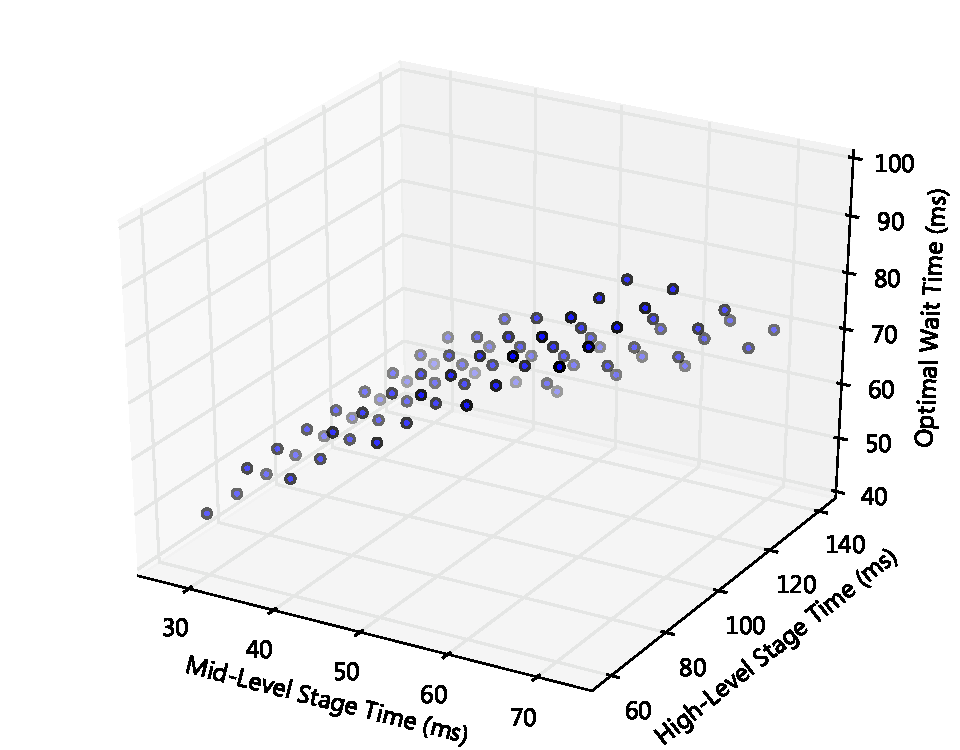
\includegraphics[width=3.2in]{../VrikshaSim/Results/07-01-2013/OptimalWaitTimes.pdf}
\caption{\small Optimal value of wait time in milliseconds for the expected values of mid-level and high-level stage times for a normal distribution across request means, and also normal distribution within a request.}
\label{figure:OptimalWaitTimes}
\end{figure}

\emph{Case 1}: The aggregators know the expected compute time for that request, i.e., it knows how expensive is the request. In this case, it picks a suitable wait time based on a priori created profile (that can be updated dynamically).
Figure~\ref{figure:OptimalWaitTimes} shows such a distribution for different value of the mean of stage distributions where these distributions are considered normal.

\begin{figure}[t]
\centering
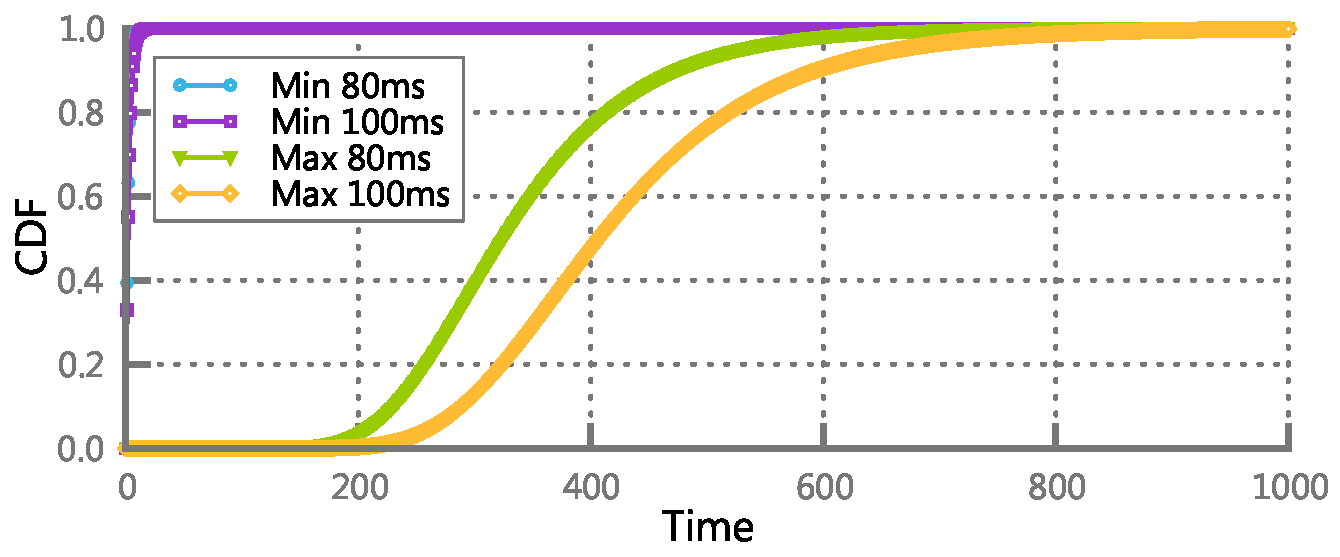
\includegraphics[width=3.2in]{Matplotlib/MinMaxExponentials.pdf}
\caption{\small CDF of exponential distribution compared against distribution of minimum and maximum of 40 exponentials}
\label{figure:MinMaxExponentials}
\end{figure}

\emph{Case 2}: The aggregator has no knowledge of the expected stage times for that request. Since, the waiting time at an aggregator that optimises for the number of worker responses included in the final response is a function of the expected stage times, the aggregator needs to estimate it somehow.
One way of doing this is to collect a few number of responses, say 10 for a fanout of 40, to get an estimate of the required information. We explain the theoretical justification below.
Consider the aggregator waiting for responses where the stage time is distributed by the random variable $X$ with a fanout of $k$. The distribution of the first response is given by 
$\textsf{min}(X^{(1)}, X^{(2)}, \dots, X^{(k)})$ and the distribution of the last response is given by
$\textsf{max}(X^{(1)}, X^{(2)}, \dots, X^{(k)})$, where $X^{(i)}$ denotes the $i^{th}$ branch. If we now compare it with another request whose stage times are distributed by $Y$, one can see that the difference between the $max$ and $min$ distributions is a good signal to distinguish between the two requests. 
Figure~\ref{figure:MinMaxExponentials} shows the CDF of the minimum and maximum for a pair of such $X$ and $Y$ that are both exponentially distributed but with different means. Thus, 
one can seek to find a good time-out on a request-to-request basis but looking at the arrival patterns of the first few responses. We leverage the concept of order statistics for this purpose as illustrated below.

\subsubsection{Order Statistics}
Consider figure~\ref{figure:2StageAggregation} for example, assuming a fan-out of $k$, denote the individual task times for the different branches to be distributed by $X^{(1)}, X^{(2)}, \dots, X^{(k)}$ assuming each one of them is identically and independently distributed. 
As stated above, the distribution of the first response is then given by 
$U = \textsf{min}(X^{(1)}, X^{(2)} \dots X^{(k)})$ while the distribution of the last response is given by $V = \textsf{max}(X^{(1)}, X^{(2)} \dots X^{(k)})$. 
Then, the CDF of $U$, $\phi_U(t) = 1 - \left[1 - \phi_{X}(t)\right]^k$ and the CDF of $V$, 
$\phi_V(t) = \left[\phi_{X}(t)\right]^{k}$. 
The $r^{th}$ order statistic is the $r^{th}$ smallest $X$ whose density function can be written 
as $p_{X_{(r)}}(t) = np_X(t)\dbinom{k - 1}{r - 1}\phi_X^{(r-1)}(t)\left(1 - \phi_X(t)\right)^{k-r}$. \notegk{If $X$ was exponentially distributed with parameter $\lambda$, the the maximum likelihood for the $r^{th}$ order statistic is achieved at $t = \frac{1}{\lambda}\ln\left(\frac{n}{n-k+1}\right)$. Thus, based on how the subsequent responses come, matching them with the corresponding MLE values, the aggregator can decide for the wait time that it should select.}
If $X$ was exponentially distributed with parameter $\lambda$, then random variable denoting the 
difference between the $r^{th}$ and $(r-1)^{th}$ order statistics is exponentially distributed with parameter $(k + 1 - r)\lambda$. One can thus estimate the $\lambda$ value incrementally by looking at the inter-arrival times of the first few responses.

\notegk{Think more?}



\section{Incremental Computation}
\notegk{2 parts}


\subsection{Response time improvements}


\section{Analytical and Simulation Results}
\subsection{Simulation}
We wrote a simulator for the partition-aggregate workflow in 3000 lines in C++. The setup consisted of a two-stage pipeline with a fan-out of 40 at each stage. We simulate 2000 requests and compute the mean values of the query quality which we assume is simply indicated by the number of responses received. 

\subsection{Same distribution for all requests}
\begin{figure}[!t]
\centering
\subfloat[Exponential Distribution] {
  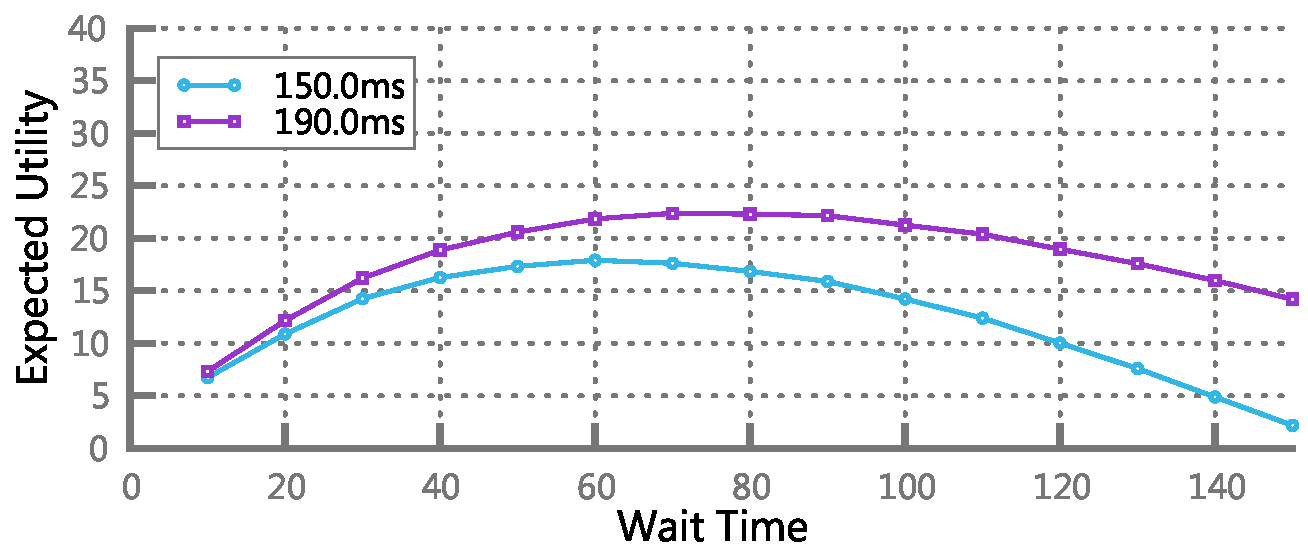
\includegraphics[width=3.1in]{Matplotlib/UtilitySimulationsExp.pdf}
  \label{figure:UtilitySimulationsExp}
}
\vspace{0.1in}
\subfloat[Normal Distribution] {
	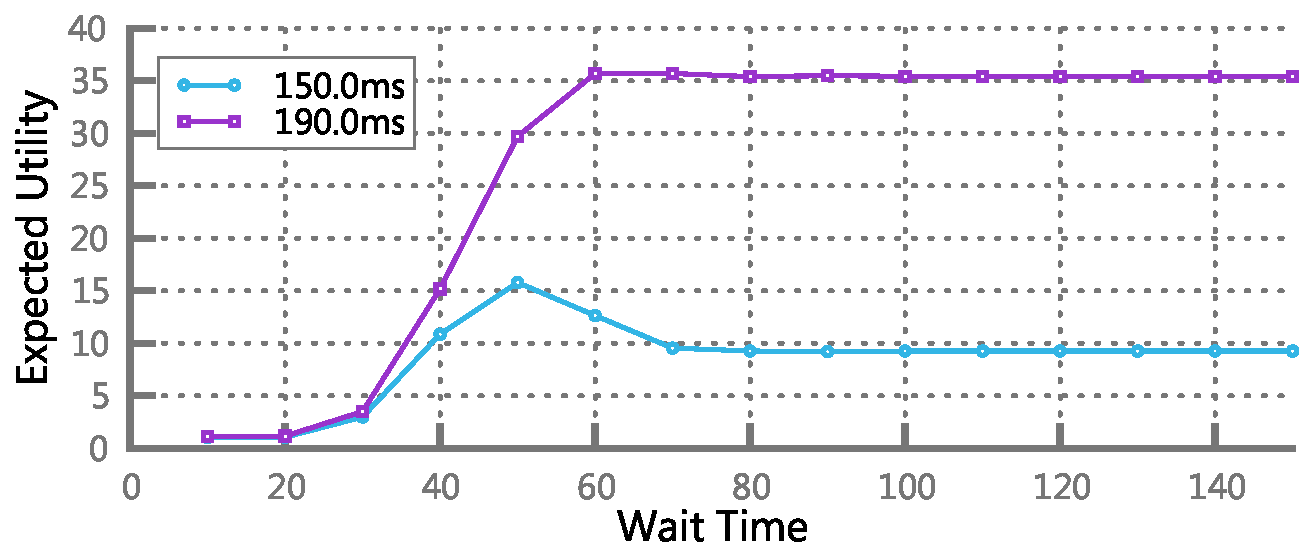
\includegraphics[width=3in]{Matplotlib/UtilitySimulationsNormal.pdf}
	\label{figure:UtilitySimulationsNormal}
}
\caption{Average value of Utility for (a) Exponential and (b) Normal distribution of stage times with different wait-times at the mid-level aggregator for deadlines of 150ms and 190ms. The mean duration for the first stage is 50ms and for the second stage is 100ms. The standard deviation for the normal distributions are 10ms for the first stage and 20ms for the second.}
\end{figure}

Figure~\ref{figure:UtilitySimulationsExp} illustrates the mean response quality where task times were picked from an exponential distribution. All the requests were equally complex and thus a single distribution was used. Figure~\ref{figure:UtilitySimulationsNormal} shows the same plot for normal distributions.

\begin{figure}[!t]
\centering
\subfloat[Response Time] {
  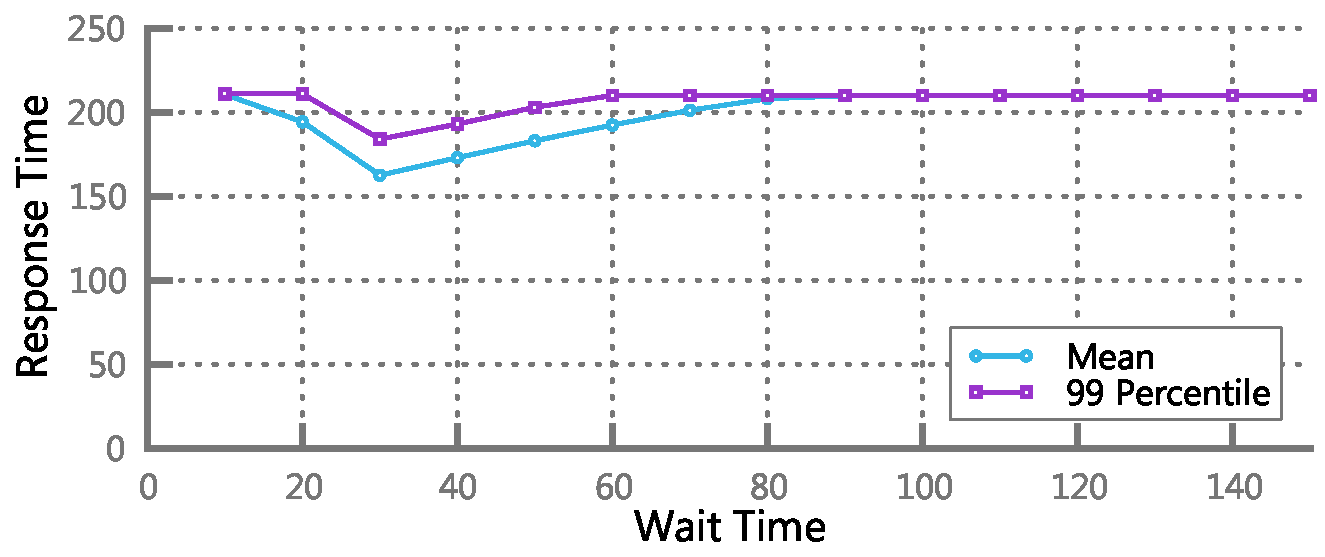
\includegraphics[width=3.1in]{Matplotlib/SimulationsNormalResponseTime.pdf}
  \label{figure:SimulationsNormalResponseTime}
}
\vspace{0.1in}
\subfloat[Utility] {
	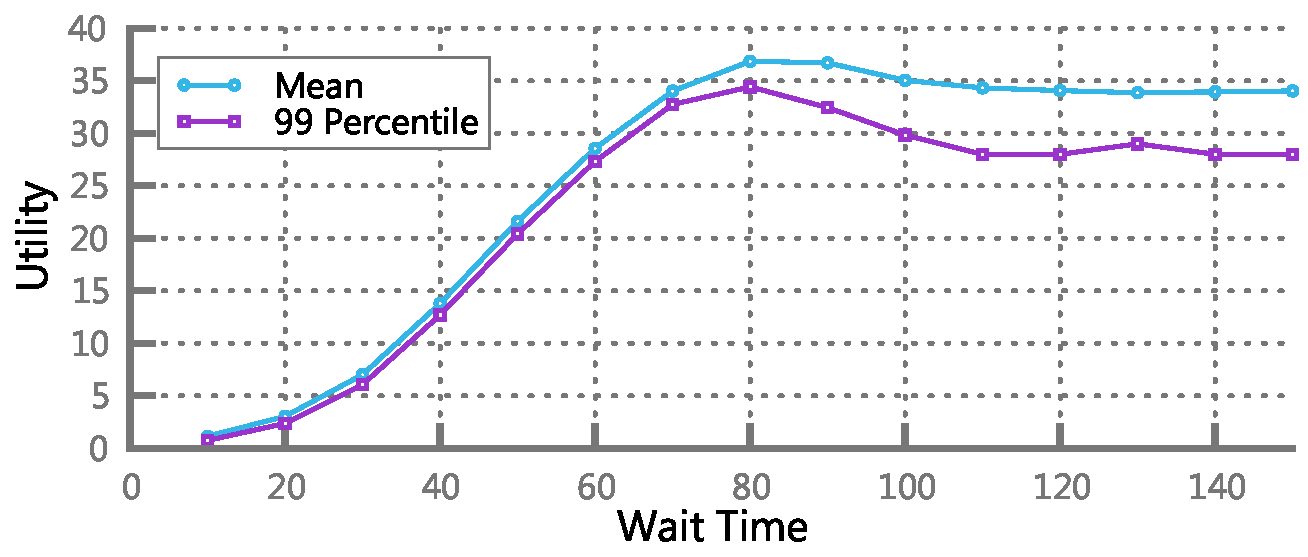
\includegraphics[width=3.1in]{Matplotlib/SimulationsNormalUtility.pdf}
	\label{figure:SimulationsNormalUtility}
}
\caption{Mean and 99 Percentile Utility and Response times for normal distribution of stage times with different wait-times at the mid-level aggregator with deadline of 210ms. The mean duration for the first stage is 50ms and for the second stage is 100ms. The standard deviation for the normal distributions are 20ms for the first stage and 15ms for the second.}
\label{figure:SimulationsNormal}
\end{figure}

We also show the effect of these timeouts on the 99 percentile values for the utility and response times in figure~\ref{figure:SimulationsNormal}.


\subsection{Optimal value more important when high variability}
\begin{figure}[!t]
\centering
\subfloat[Mean Utility] {
  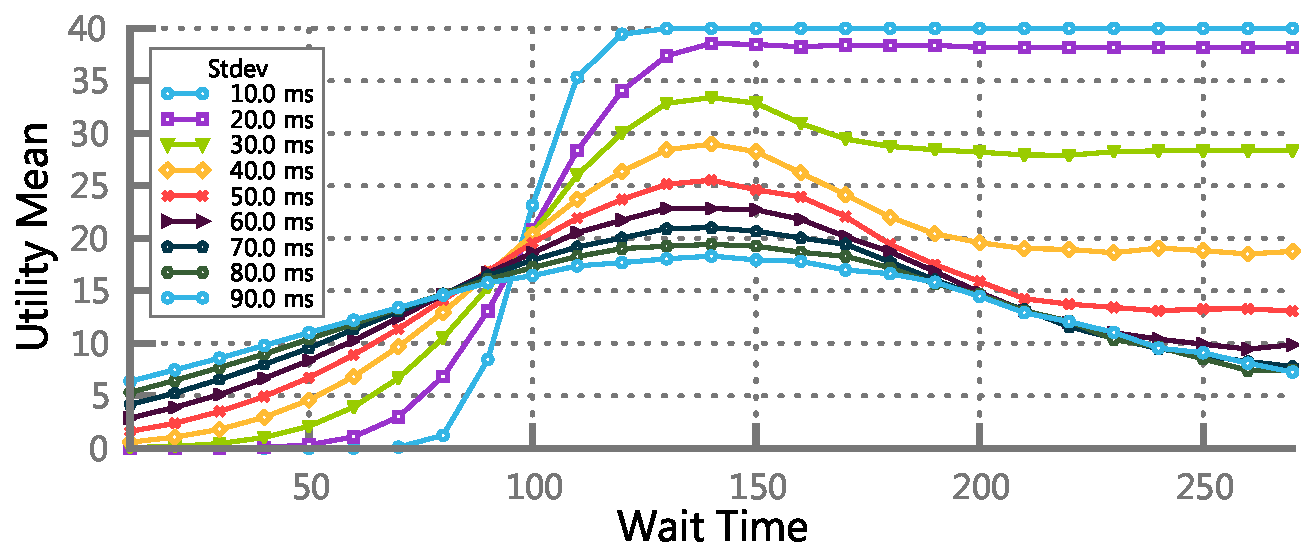
\includegraphics[width=3.1in]{../VrikshaSim/Results/07-01-2013/OptimalWrtStdevMeanNormal.pdf}
  \label{figure:OptimalWrtStdevMeanNormal}
}
\vspace{0.1in}
\subfloat[99 percentile Utility] {
	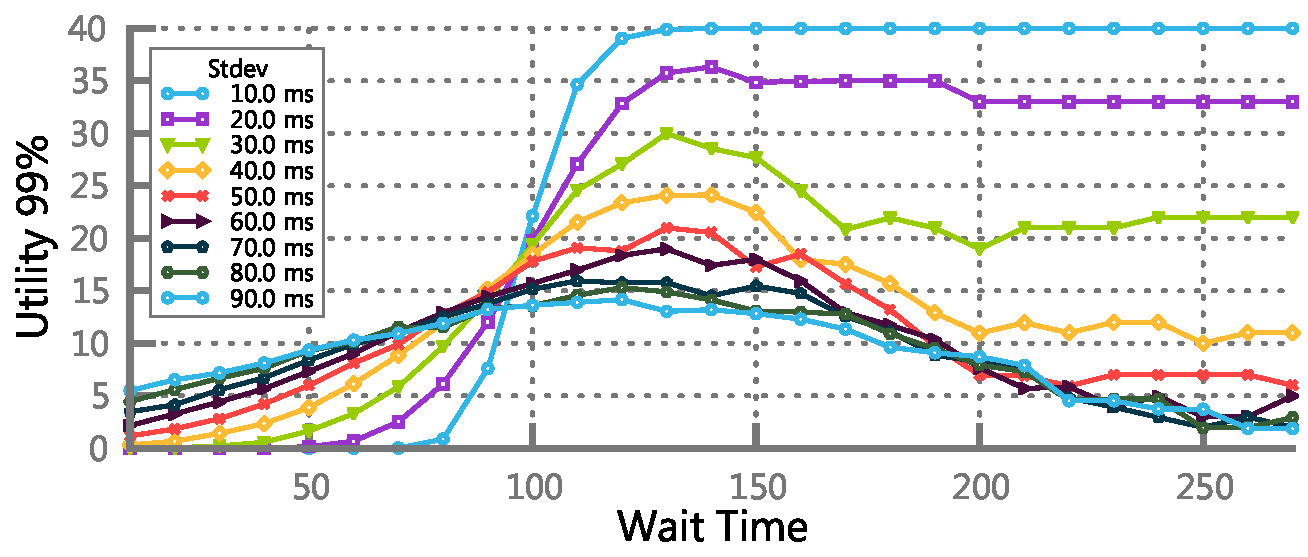
\includegraphics[width=3in]{../VrikshaSim/Results/07-01-2013/OptimalWrtStdev99Normal.pdf}
	\label{figure:OptimalWrtStdev99Normal}
}
\caption{Normally distributed -- Utility values as a function of wait time at the mid-level aggregator for different values of standard deviation of task distributions.}
\label{figure:OptimalWrtStdevNormal}
\end{figure}


\begin{figure}[!t]
\centering
\subfloat[Response Time] {
  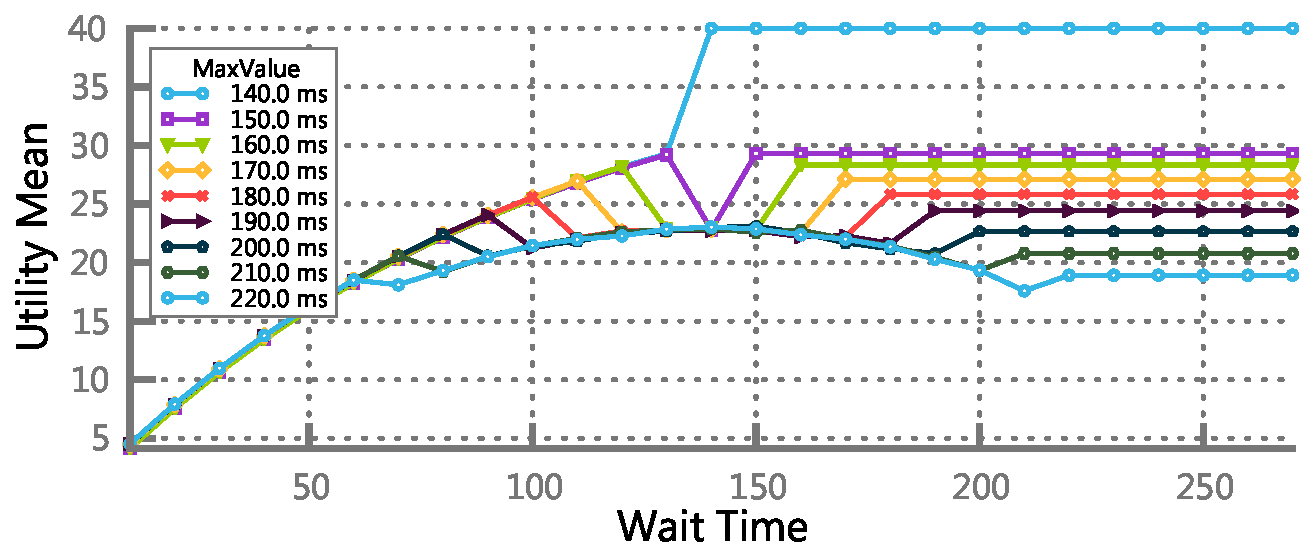
\includegraphics[width=3.1in]{../VrikshaSim/Results/07-01-2013/OptimalWrtMaxValueMeanExp.pdf}
  \label{figure:OptimalWrtMaxValueMeanExp}
}
\vspace{0.1in}
\subfloat[Utility] {
	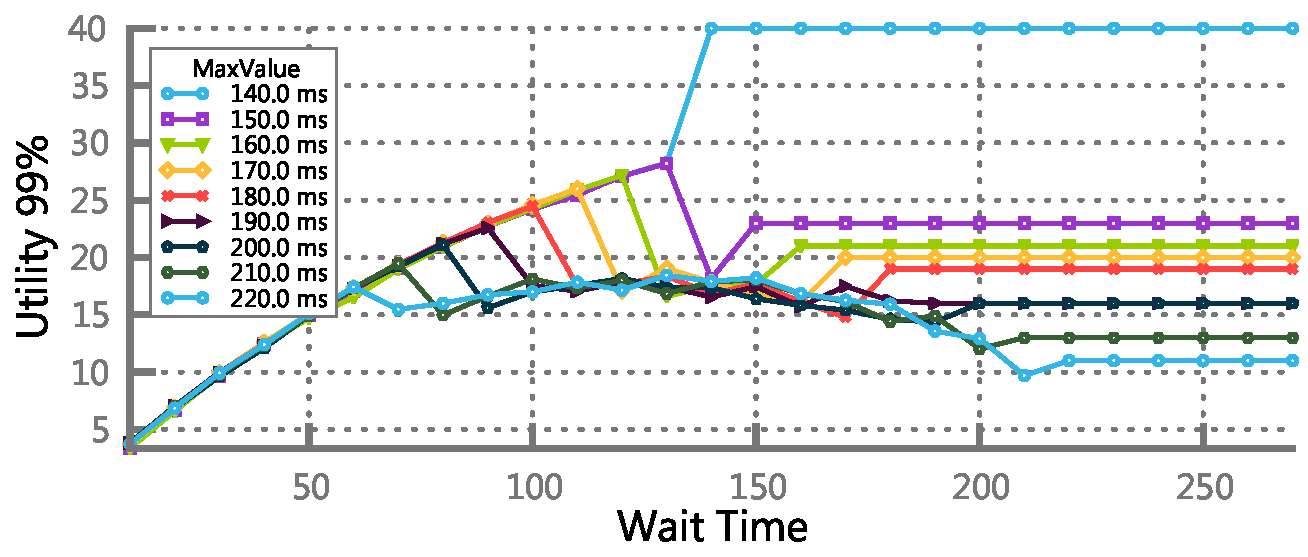
\includegraphics[width=3in]{../VrikshaSim/Results/07-01-2013/OptimalWrtMaxValue99Exp.pdf}
	\label{figure:OptimalWrtMaxValue99Exp}
}
\caption{Exponentially distributed -- Utility values as a function of wait time at the mid-level aggregator for different values of max values of task distributions.}
\label{figure:OptimalWrtMaxValueExp}
\end{figure}
One can see, that selecting an optimal value for the timeout becomes more important as the system has more variance in task times distributions. To this effect, we consider the following two cases, one where the distributions are gaussian and we vary the standard deviation to induce more variance in the system. The second, when the underlying task durations are exponentially distributed but we chop it off at an upper bound and vary this upper bound. Figure~\ref{figure:OptimalWrtStdevNormal} and Figure~\ref{figure:OptimalWrtMaxValueExp} plot how the utility values change for different amounts of variability in the system. It is important to note that the criticality of timeout selection is dependent on how much variability exists in the system.

\begin{figure}[t]
\centering
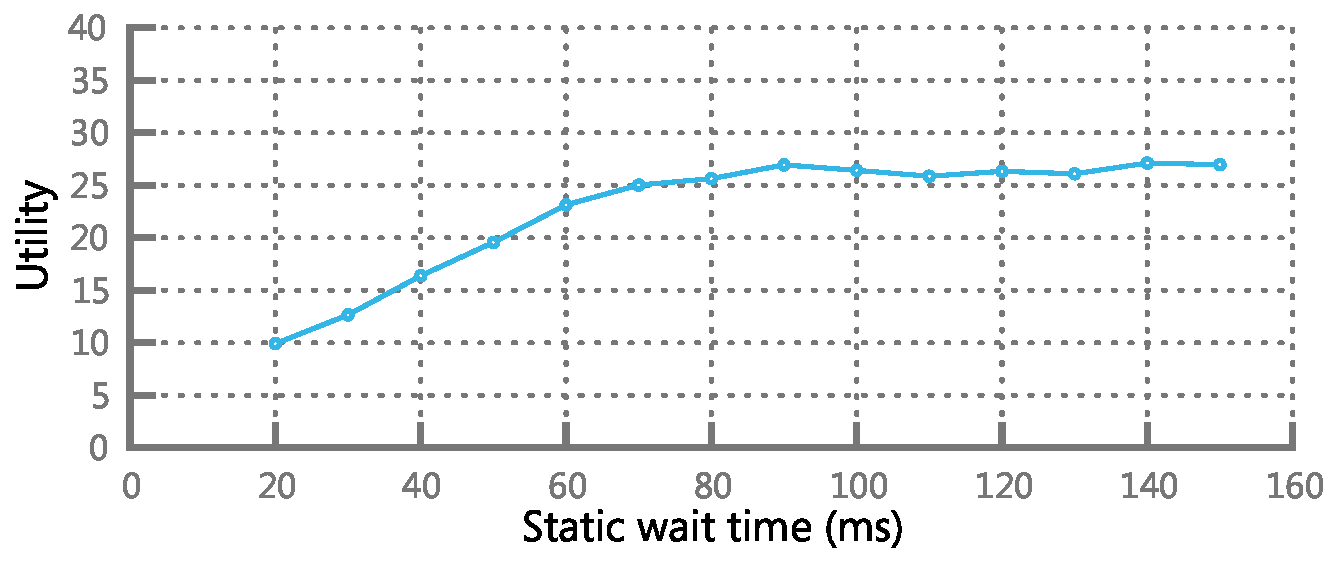
\includegraphics[width=3.2in]{../VrikshaSim/Results/07-01-2013/StaticWaitTimes.pdf}
\caption{Utility values for different value of static wait times for a normal distribution across request means, and also normal distribution within a request.}
\label{figure:StaticWaitTimes}
\end{figure}

\subsection{Different distribution for all requests}
In this section, we compare how the dynamic waiting-time scheme contrast against static time-outs. Figure~\ref{figure:StaticWaitTimes} shows the expected utility as a function of the static timeout.


\subsection{Experiments}
We implemented a simple web-search application on Amazon EC2 using 100 machines in Python.
\notegk{results from experiments}.


In contrast, the dynamic timeout policy achieves a near utility of 26.51, but completes 941 requests compared to the 869 requests that the maximum utility static timeout achieves (27.12).

\section{Trace-driven Analysis}
\notegk{Experiments from trace-driven simulations, if possible.}


{\footnotesize \bibliographystyle{acm}
\bibliography{../common/bibliography}}


\theendnotes

\end{document}






